%%%%%%%%%%%%%%%%%%%%%%%%%%%%%%%%%%%%%%%%%%%%%%%%%%%%%%%%%%%%%%%%%%%%%%%%%%%
%% This file is part of the book
%%
%% Algorithmic Graph Theory
%% http://code.google.com/p/graph-theory-algorithms-book/
%%
%% Copyright (C) 2009, 2010 Minh Van Nguyen <nguyenminh2@gmail.com>
%%
%% See the file COPYING for copying conditions.
%%%%%%%%%%%%%%%%%%%%%%%%%%%%%%%%%%%%%%%%%%%%%%%%%%%%%%%%%%%%%%%%%%%%%%%%%%%

\subfigure[]{
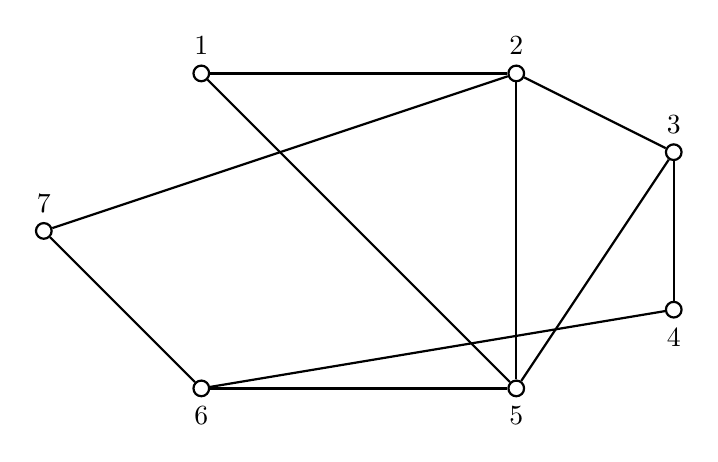
\begin{tikzpicture}
[nodedecorate/.style={shape=circle,inner sep=2pt,draw,thick},%
  linedecorate/.style={-,thick}]
%% nodes or vertices
\foreach \nodename/\x/\y/\direction/\navigate in {2/4/4/above/north,
  1/0/4/above/north, 3/6/3/above/north, 4/6/1/below/south,
  5/4/0/below/south, 7/-2/2/above/north, 6/0/0/below/south}
{
  \node (\nodename) at (\x,\y) [nodedecorate] {};
  \node [\direction] at (\nodename.\navigate) {$\nodename$};
}
%% edges or lines
\path
\foreach \startnode/\endnode in {1/2, 1/5, 2/3, 2/5, 2/7, 3/4, 3/5,
  4/6, 5/6, 6/7}
{
  (\startnode) edge[linedecorate] node {} (\endnode)
};
\end{tikzpicture}
}
%%
%%
\qquad
\subfigure[]{
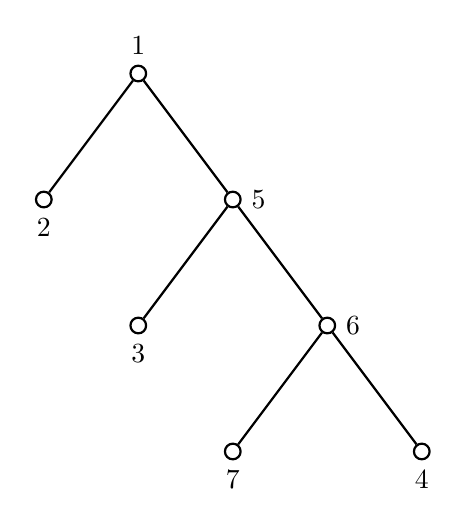
\begin{tikzpicture}
[nodedecorate/.style={shape=circle,inner sep=2pt,draw,thick},%
  linedecorate/.style={-,thick},%
  scale=1.6]
%% nodes or vertices
\foreach \nodename/\x/\y/\direction/\navigate in {
  1/1.25/3/above/north, 2/0.5/2/below/south, 5/2/2/right/east,
  3/1.25/1/below/south, 6/2.75/1/right/east, 7/2/0/below/south,
  4/3.5/0/below/south}
{
  \node (\nodename) at (\x,\y) [nodedecorate] {};
  \node [\direction] at (\nodename.\navigate) {$\nodename$};
}
%% edges or lines
\path
\foreach \startnode/\endnode in {1/2, 1/5, 3/5, 5/6, 6/7, 6/4} {
  (\startnode) edge[linedecorate] node {} (\endnode)
};
\end{tikzpicture}
}
%%
%%
\subfigure[]{
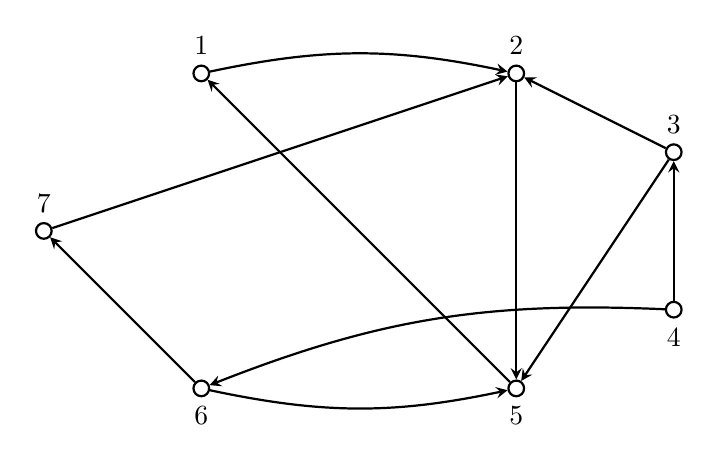
\begin{tikzpicture}
[nodedecorate/.style={shape=circle,inner sep=2pt,draw,thick},%
  arrowdecorate/.style={->,>=stealth,thick}]
%% nodes or vertices
\foreach \nodename/\x/\y/\direction/\navigate in {2/4/4/above/north,
  1/0/4/above/north, 3/6/3/above/north, 4/6/1/below/south,
  5/4/0/below/south, 7/-2/2/above/north, 6/0/0/below/south}
{
  \node (\nodename) at (\x,\y) [nodedecorate] {};
  \node [\direction] at (\nodename.\navigate) {$\nodename$};
}
%% edges or lines
\path
\foreach \startnode/\endnode in {2/5, 3/2, 3/5, 4/3, 5/1, 6/7, 7/2} {
  (\startnode) edge[arrowdecorate] node {} (\endnode)
}
\foreach \startnode/\endnode/\benddirection/\angle in {
  1/2/bend left/12, 4/6/bend right/12, 6/5/bend right/12}
{
  (\startnode) edge[arrowdecorate,\benddirection=\angle] node {} (\endnode)
};
\end{tikzpicture}
}
%%
%%
\qquad
\subfigure[]{
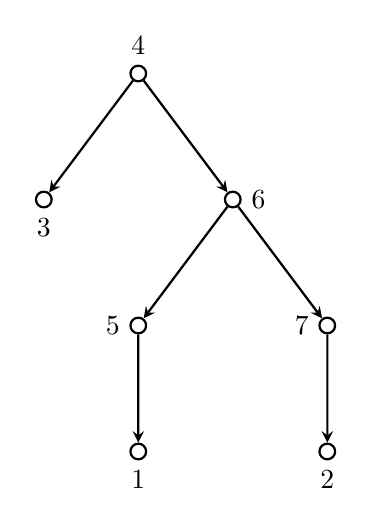
\begin{tikzpicture}
[nodedecorate/.style={shape=circle,inner sep=2pt,draw,thick},%
  arrowdecorate/.style={->,>=stealth,thick},
  scale=1.6]
%% nodes or vertices
\foreach \nodename/\x/\y/\direction/\navigate in {
  4/1.25/3/above/north, 3/0.5/2/below/south, 6/2/2/right/east,
  5/1.25/1/left/west, 7/2.75/1/left/west, 1/1.25/0/below/south,
  2/2.75/0/below/south}
{
  \node (\nodename) at (\x,\y) [nodedecorate] {};
  \node [\direction] at (\nodename.\navigate) {$\nodename$};
}
%% edges or lines
\path
\foreach \startnode/\endnode in {4/3, 4/6, 6/5, 6/7, 5/1, 7/2} {
  (\startnode) edge[arrowdecorate] node {} (\endnode)
};
\end{tikzpicture}
}
